
\documentclass[11pt,english,a4]{article}

\topmargin = 5 mm
\oddsidemargin = 0mm
\evensidemargin = 0mm
\headheight = 0 mm
\headsep = 0 mm
\textheight = 220 mm
\textwidth = 157 mm
 
% for 1 inch margins all around.
 
\usepackage{doublespace}
\usepackage[pdftex]{graphicx}

\title{Quality-Attribute Driven Organizational Architecture}
\author{Friedemann (Fritz) Solms \\ Solms Training, Consulting \& Development \\
        PostNet Suite 237, Private Bag X9, Melville, 2109, South Africa \\
				E-Mail: fritz@solms.co.za, Tel: +27 11 646 6459, Fax: +27 11 646 5868}

\begin{document}
\maketitle

\begin{abstract}
	This article suggests that organizational business process design and architecture are orthogonal. While the former addresses the core functional requirements of client use cases, the latter ensures that the organizational qualities are manifested across the business processes realizing the client use cases. Furthermore, the article proposes a method for designing and analyzing an organization's architecture from the perspective of its quality attributes.  Common architectural patterns like hierarchical, pipes and filters, expert pools and franchises are analyzed on their capability to realize core quality requirements. For each quality attribute common realization strategies are explored. Ultimately an organization's architecture is assembled from a combination of architectural patterns and strategies as to effectively realize its vision. 
\end{abstract}

\section{Introduction}

Increasingly, organizational architecture is key to managing a modern organization in such a way that it remains aligned with its vision. The vision statement is used to publish the core organizational qualities defining the essence of the organization. Some organizations see their core quality as reliability, while others may aim to differentiate themselves through, for example, ingenuitivity, flexibility, scaleability, or availability. Often it is these quality attributes which provide an organization its competitive edge.

The organizational architecture provides the framework within which the business processes are deployed. It ensures the organization's core qualities are consistently realized across the various business processes and provides the basis for high-level decision making and metrics.

A number of authors have looked at organizational architecture (see, for example
 \cite{Ashmore-Henson-Chancellor-Nelson-2004},
 \cite{Brickley-Smith-Zimmermann-2001},
 \cite{Nadler-Gerstein-Shaw-1992},
 \cite{Galbraith-Downy-Kates-2001},
 \cite{Ethiraj-Levinthal-2004}. Some like \cite{King-1995} and to some extend \cite{Ashmore-Henson-Chancellor-Nelson-2004} suggested that organizational architecture should be driven by the organization's strategic vision and should realize the organization's capabilities.

This article aims to put this vision into practice. The approach starts by looking at an organization's vision in order to identify its core quality goals. Next one investigates a suitable architectural foundation by looking at how one can combine proven architectural patterns to define the course-grained organizational architecture. Having specified the structural foundation for the architecture, one now needs to look at strategies which will be used to concretely realize the various quality goals of the organization across its various business processes. The organization's architecture is ultimately assembled from a particular combination of architectural patterns and strategies.

\section{What are quality attributes of an organization?}

Some organizations, particularly in the high-technology field, view ingenuitivity as their core value offering. Others provide services to mission critical areas like the health or aerospace industries. Such organizations may target reliability as the core quality attribute. Yet others may extract value from low cost products or services through high volumes. They would be concerned with realizing scalability.

Quality attributes thus define an organization's core capabilities. These capabilities should be evident across the organization's business processes and hence represent intrinsic qualities around the services it offers to its clients. The organizational qualities are typically expressed in the {\em{Vision Statement}} of the organization.

For example, the vision statement of our little organization, Solms Training, Consulting \& Development, reads as follows: 
\begin{quote}
	{\em{To provide innovative and customizable training, consulting and development services which assist our clients to gain a competitive edge. We focus on organizational and system architecture, business process design and realization as well as quality assurance on any of these.}}
\end{quote}

The vision statement quotes the core quality attributes as
\begin{description}
	\item[innovation],  enabling us to come up with novel solutions which
        may assist our customers to gain a competitive edge, and
	\item[flexibility/customizability] which enables us to customize our services (e.g.\ the course contents) to address our customers specific needs.
\end{description}
\noindent  These qualities should be present across the training, consulting and development services offered by the organization. It is the organizational architecture which needs to provide the infrastructure to realize these qualities across our services.

Another organization may state in its vision the ability to provide standardized, accredited courses to a huge number of clients across the world. The core qualities may be {\em{scaleability}} and {\em{availability}}. The architectures of the two organizations are bound to be very different. The latter organization could perhaps use role-based human resourcing, replication, outsourcing (for the taking of exams), fixed, rigidly defined workflows and potentially a combination of hierarchical and pipes-and-filters based structural elements in the organization's architecture.

However, this would most likely not work for our organization whose core qualities are innovation and modifiability. Instead we use person-centric human resourcing encouraging staff members to define and evolve their own role within the organization. Furthermore, the core of the organization's architecture facilitates innovation via an expert pool (using the blackboard architectural pattern discussed later) embedded within a very flat hierarchy.

\section{What is organizational architecture?}

The architecture of an organization is its high-level (course grained) structure, the procedural framework for its business processes, and the communication strategies used internally between the business units and externally to its clients and business partners. 

Business processes used to realize the client services may change quite frequently in order to address changing client needs and new business opportunities. Organizational architecture, on the other hand, should change much less frequently, largely only when the organization's vision is re-aligned.

In software development circles it is well understood that system architecture is largely driven by the non-functional system requirements, i.e. the required quality attributes for the system. The detailed functional requirements around individual use case generally have little impact on the system architecture (see, for example, \cite{Bass-Clements-Kazman-2003} and \cite{Kazman-1994}).

Here we argue that organizational architecture should similarly be driven by the core qualities which define the essence of the organization. Such an approach facilitates that these qualities will be addressed across the business processes of the organization and hence across the services it offers.


\section{Organizational architecture versus business process design}

The architecture of an organization realizing the organization's quality attributes is largely independent of the business processes deployed within that architecture. Furthermore, one can even define the business processes in an architecture/deployment environment neutral way and then map the generic business processes onto defined business processes as realized within a specific architecture. 

Note that this approach is equivalent to the {\em{Model Driven Architecture}} (MDA, see for example \cite{Frankel-2003}) as published by the Object Management Group (OMG). In the context of MDA the architecture-neutral design (e.g. business process design) is called the {\em{Platform-Independent Model}} (PIM). The PIM is then mapped into a deployment architecture resulting in the {\em{Platform Specific Model}} (PSM).

\section{Architectural patterns}

The use of patterns as generic design solutions has been pioneered by Christopher Alexander (see \cite{Alexander-1979}). Alexander applied architectural patterns as reusable solutions to buildings architecture.

Software designers and architects soon found that they too could benefit from basing their systems on proven generic architectural and design solutions. The most renowned publication around software design patterns is the so-called {\em{``Gang of four book''}} \cite{Gamma-Helm-Johnson-Vlissides-1995} which lists 35 patterns addressing various common software design problems in a simple and elegant way.

This article similarly argues that management and business analysts can benefit substantially from using proven architectural patterns to improve their organizational architecture. Patterns for organizational architecture provide generic, proven ways in which an organization's core quality attributes can be realized.

Different architectural patterns address different core quality attributes. For example, the pipes and filters pattern promotes modifiability. It is frequently used by organizations which regularly need to modify their workflows to address their client's particular and/or changing needs.

The architecture for an organization will typically be assembled from a combination of architectural patterns. Often a specific pattern specifies the core structure of the organization. That pattern should be aligned with the core desired quality attribute for that organization. Further architectural patterns can be used to adress other quality attributes. The specific combination of architectural patterns and strategies define the architecture for that organization. It is this architecture which, in many cases, gives the organization its competitative edge.

Below we select a few architectural patterns to illustrate the concepts.

\subsection{The hierarchical pattern}

Traditionally most large enterprises were architected around the hierarchical pattern. Over the last few decades the tendency has been to move away from deep hierarchical structures to more flat team-based organizations. However, most of these more flat organizational structures are still hierarchical in their core (see, for example \cite{Leavitt-2004}). In the extreme these organizations represent a single-level hierarchy.

\begin{figure}[hbt]
  \begin{center}
    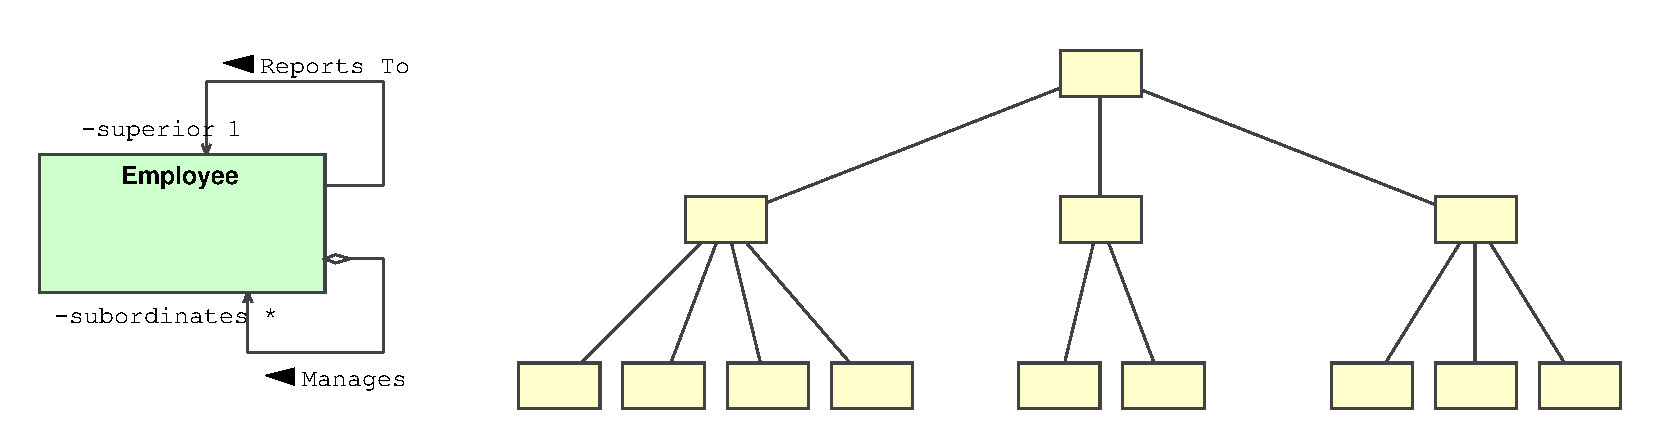
\includegraphics[scale=0.4]{hierarchicalStructure}
    \caption{The structure of a hierarchical architecture}\label{hierarchicalStructure_fig}
  \end{center}
\end{figure}

\subsubsection{Vision of the hierarchical pattern}

The theory behind hierarchical organizations is that an individual's position within the organization evolves such that the individual grows into the domain of responsibility they would like to and are able to handle (see, for example, \cite{Harris-Raviv-2002}). A position within the hierarchy thus represents a domain of responsibility.

Communication within a hierarchical organization is restricted to 
\begin{itemize}
  \item communication within the domain at that hierarchical level,
  \item communication to the next lower level in the hierarchy (the subordinates),
  \item communication to the immediate superior, and
  \item service requests to other business units along well defined client/server routes.
\end{itemize}
\noindent 
The hierarchical pattern combines vertical layering with horizontal partitioning: 
\begin{itemize}
  \item The vertical layering takes one to higher and higher levels of workflow management and decision making resulting in an accountability hierarchy.
  \item The horizontal partitioning into separate business units with their own domains of responsibility results in responsibility localization.
\end{itemize}

\subsubsection{Human resourcing in hierarchical organizations}

Since hierarchical organizations divide the domain into well-defined areas of responsibility, they typically favour role-based human resourcing, i.e. individuals are hired to fill a well defined role within the organization.

\subsubsection{Strengths of hierarchical organizations}

Hierarchical organizations have proven themselves over a long time. This architectural pattern can be expected to remain a widely used pattern in the enterprise world for some time to come. The core reasons for this are: 
\begin{itemize}
  \item Hierarchical architectures encourage responsibility localization at various levels of granularity.
  \item They reduce the number of communication paths within an organization and hence the complexity of a large organization.
  \item Hierarchical organizations scale well.
\end{itemize}

\subsubsection{Weaknesses of hierarchical organizations}

However, many organizations have started to break down their hierarchical structures. They find that the reduced communication channels becomes more of a liability than an asset. Disadvantages of hierarchical structures include the following: 
\begin{itemize}
  \item Hierarchical organizations tend to be very rigid, i.e.\ modifying business processes or introducing new 
         business processes can be quite costly, particularly if responsibility allocations need to be changed.
  \item Deep hierarchies discourage ingenuitivity and personal development.
  \item The rigid demarcation of areas of responsibility discourages taking initiatives which fall outside the allocated area of responsibility.
  \item If the transition to higher levels within the hierarchy is not managed carefully then it may easily happen that individuals are promoted until they cannot cope with the allocated level of responsibility, i.e. until they have settled in their level of incompetence.
  \item It is difficult to support a paradigm where individuals define and evolve their own role within the organization. This is partially due to the partitioning into separate areas of responsibility and partially due to the restricted communication across accountability layers.
  \item The horizontal domain partitioning can easily result in stove-pipes where communication across business units deteriorates over time. This typically results in workflow and responsibility duplication across the organization. Furthermore, evolving the business and changing business processes in a way which remains aligned to the organization's vision and quality attributes becomes difficult. Stove pipes are also often directly created by mergers.
\end{itemize}

\subsubsection{Hierarchical architectures and quality attributes}

Strong hierarchical architectural structures are typically favoured by large organizations whose core qualities include scaleability, accountability and to a lesser extend by organizations which have reliability.

On the other hand, if the core qualities of an organization include ingenuitivity and modifiability then one typically wants to reduce the hierarchical elements within the organization.

\subsection{The blackboard pattern}

Many modern organizations, particularly in the knowledge and technology fields, regard ingenuitivity as their core quality attribute. Such companies are often architected around the blackboard pattern.

The core elements of the blackboard architectural pattern are 
\begin{itemize}
  \item an expert pool,
  \item the organization's knowledge base (the blackboard), and
  \item management which plays the role of controller.
\end{itemize}
\noindent  
Organizations built around the blackboard pattern have in their core a dynamic, evolving expert pool. The experts within this pool typically define and evolve their own role within the organization. They select themselves when and how they can best contribute to problems the organization is working on.

\begin{figure}[hbt]
  \begin{center}
    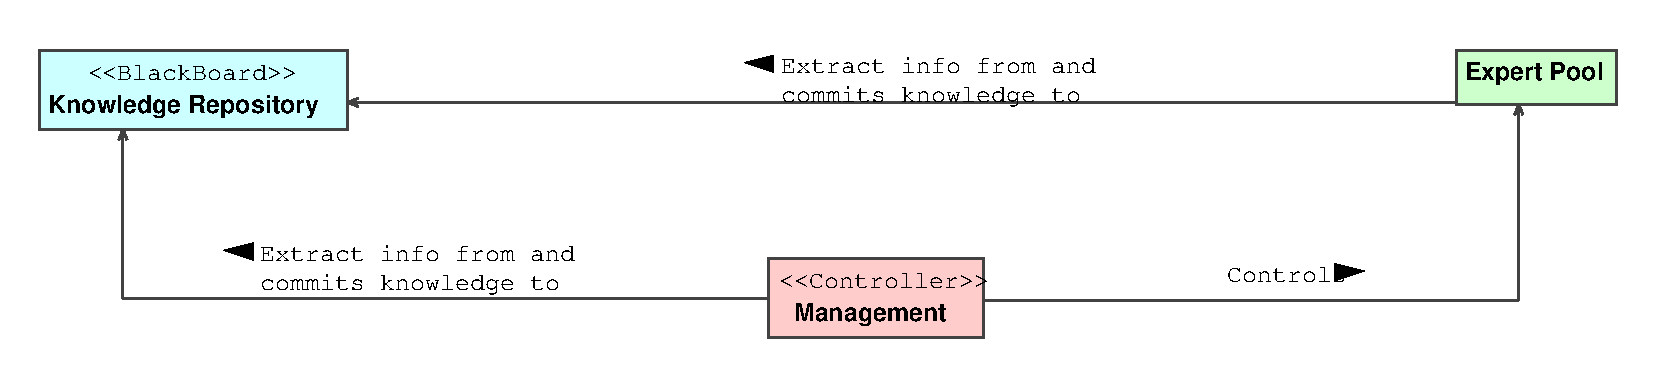
\includegraphics[scale=0.4]{blackboardStructure}
    \caption{The structure of a blackboard-based architecture}\label{blackboardStructure_fig}
  \end{center}
\end{figure}

It is important that the body of knowledge continuously grows and that it is accessible to all experts. To this end the organization uses a knowledge repository (the blackboard) which maintains the current knowledge within the organization, the problems the organization is and has been working on, as well as the current state of the solutions to the various problems.

Management controls these collaborative problem solving processes. It 
\begin{itemize}
  \item provides a suitable environment for the experts to effectively operate and grow,
  \item feeds problems to experts who are in a position to meaningfully contribute,
  \item and facilitates a process of selecting the best contribution towards a solution.
\end{itemize}
\noindent  
Note that open source software development uses the blackboard architectural pattern. The open source developers are the domain experts. They select themselves when and how they can best contribute. A controller selects the best contribution. The software source and documentation represent the knowledge repository (blackboard). Experts perform quality assurance on each other. (In some examples like the community driven encyclopedia, WikiPedia, anybody can directly add to the blackboard and the community as a whole selects what should be removed from the blackboard.)

\subsubsection{Recursive blackboards}

One of the novelties of the blackboard pattern is that it can be applied recursively. For example, consider the following two-layer blackboard. At the lower level core areas of responsibility may be addressed within separate business units some or all of which may be using the blackboard architecture. In the second level management decisions are done via an expert pool with the experts being the managers of the individual business units and the controller being the managing director of the company.

\subsubsection{Human resourcing in the context of blackboard based organizational architectures}

Blackboard based architectures typically use person-centric human resourcing where a person is not hired for a particular role, but instead defines and evolves his or her own role within the organization. For organizations thriving on ingenuitivity it is key to ensure that experts continue to grow by exposing them to ever more challenging problems and to different environments.

\subsubsection{Strengths of the blackboard architectural pattern}

As stated previously, the pattern is particularly attractive for organizations driven by ingenuitivity. Its strengths include: 
\begin{itemize}
  \item An environment where individuals define and evolve their own role within the organization encourages enthusiasm and initiative.
  \item Continuous, intrinsic quality assurance across experts results in higher quality solutions and reduced risk.
  \item Providing an environment for natural growth and evolution usually results in lower staff turnover and hence better knowledge retention.
  \item The capability of the organization grows continuously.
  \item The blackboard pattern provides a framework for solving difficult problems.
  \item A knowledge repository captures and maintains knowledge within the organization.
\end{itemize}

\subsubsection{Weaknesses of the blackboard pattern}

Though the blackboard pattern is great for driving ingenuitivity and quality, it does introduce a few issues which need to be managed: 
\begin{itemize}
  \item Lack of responsibility allocation results in weak accountability tracing and requires additional processes which ensure that all responsibilities are ultimately attended to.
  \item Collaborative quest for best solution may result in weak performance.
  \item Exposure to individual capabilities and losing certain individuals may significantly impact the organization.
  \item Cost implications of active redundancy, i.e. multiple experts work on the same problem.
\end{itemize}

\subsubsection{The blackboard pattern and quality attributes}

Organizations will typically assemble an architecture using a combination of architectural patterns. Organizations which make heavy use of the blackboard pattern typically see ingenuitivity and modifiability as their core quality attributes.

Organizations which view their core qualities as accountability, scaleability, reliability and performance will typically use the blackboard pattern in only very confined areas like R\&D.

\subsection{Dynamic workflows via pipes and filters}

Organizations which see modifiable workflows as one of their core qualities often make extensive use of the pipes and filters pattern. Here business units take over the responsibility of individual workflow steps. Business processes are defined as workflows across these business (processing) units. The idea is that one can very easily assemble and modify business processes within this architecture. Pipes and filters based architectures aim for workflow based horizontal integration across responsibility domains.

\begin{figure}[hbt]
  \begin{center}%
    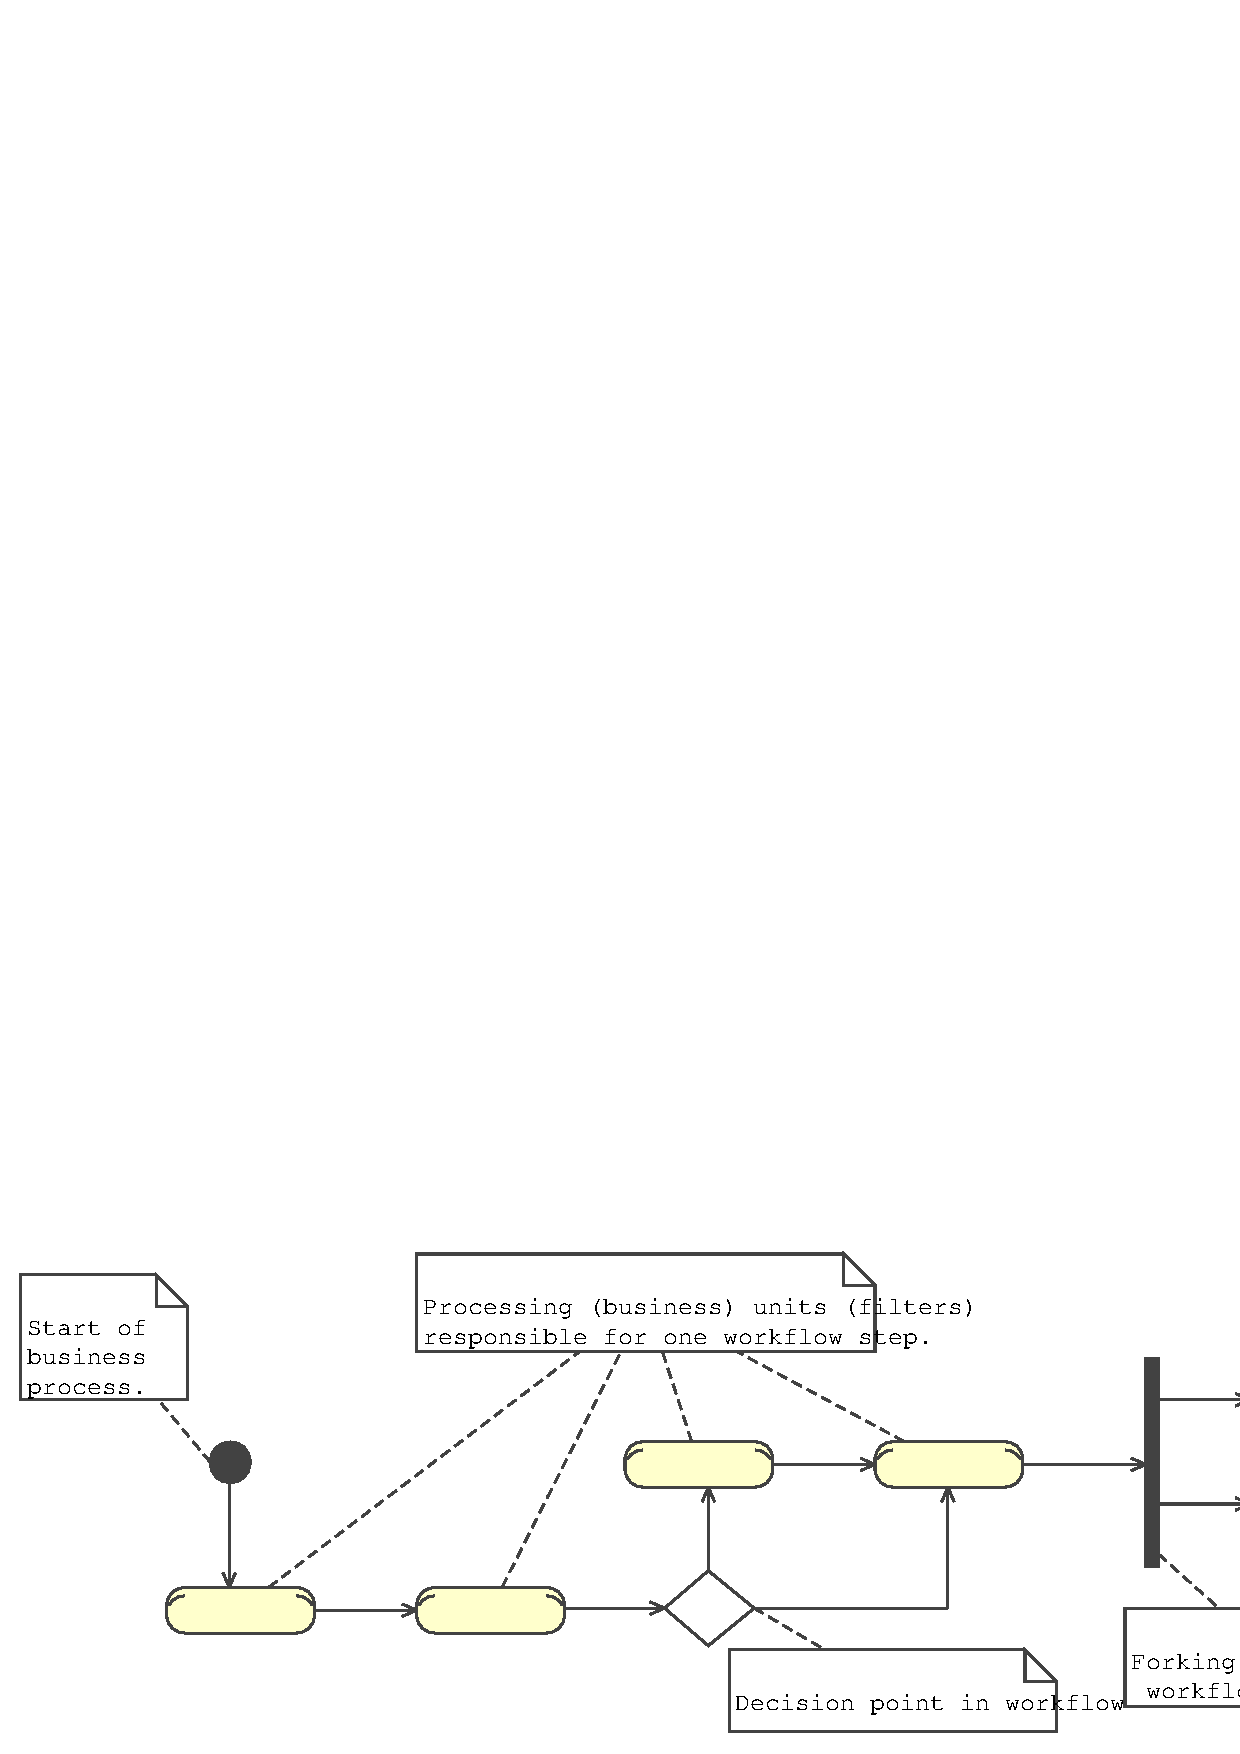
\includegraphics[scale=0.4]{pipesAndFiltersExample}
    \caption{Realizing business processes in a pipes and filters based architecture.}
		\label{pipesAndFiltersExample_fig}
  \end{center}
\end{figure}

When setting up a pipes and filters architecture one needs to start with a clean responsibility allocation across business units. With each business unit responsible for a particular processing step one assembles workflows across these. One then needs to put an optimized communication infrastructure in place which typically requires support for queueing and guaranteed delivery. A common solution for this is a services bus which integrates the business units across the organization.

\subsubsection{Management structure for a pipes and filters based organization}

Managing large pipes and filters based organizations is non-trivial. Traditionally one would tend to put a hierarchy on top of the pipes and filters structure which is based on domains of responsibility, i.e. based on a groupings of the processing units.

However, since workflows are typically constructed across these domains of responsibility, this does not result in effective workflow management. The higher level accountability should reside in a relatively flat hierarchy based on a services and hence workflow categorization. This results in direct workflow ownership at various levels of abstraction and results in accountability based on the services one offers to one's clients.

\subsubsection{Human resourcing from a pipes and filters perspective}

Due to the strong responsibility localization and the workflow centric approach of pipes and filters based organizational architectures they generally tend to use role-based human resourcing.

\subsubsection{Strengths of the pipes and filters pattern}

Workflow-centric organizations often make heavy use of the pipes and filters architectural pattern. Core benefits include 
\begin{itemize}
  \item One can easily and rapidly assemble new workflows.
  \item One can easily modify existing workflows.
  \item The pipes and filters pattern typically results in good responsibility localization across the organization.
  \item Scaleability and reliability is easily achieved through replication of processing units.
\end{itemize}

\subsubsection{Weaknesses of the pipes and filters pattern}

If the core desired quality attribute for your organization is ingenuitivity, then you would typically want to minimize architectural features based on the pipes and filters pattern. The strong focus on roles within the organization tends to discourage individual initiatives and ingenuitivity.

\subsection{The franchise pattern}

The number of organizations which use the franchise as the core architectural pattern for their organization has grown rapidly over the past few decades. Franchises typically see their core qualities in the ability to leverage capital investments and the opportunities for rapid growth.

When setting up a franchise one needs to put the support structure for the franchisees in place. This typically includes 
\begin{itemize}
  \item the establishment of a franchise brand and the infrastructure to maintain and grow the brand,
  \item the infrastructure for product and market research as well as general marketing,
  \item the infrastructure for bulk purchasing and distribution,
  \item training channels for franchisees,
  \item the business support structures for the franchisees,
  \item the infrastructure to perform QA on franchisees,
  \item feedback channels incorporating field-based ideas originating from franchisees, and
  \item the infrastructure to collect revenue from the franchisees.
\end{itemize}
\noindent 
For many of these elements other architectural patterns are employed. For example the core architecture within the franchiser organization may be hierarchical. However, within that hierarchical structure the organization may use the blackboard pattern for the R\&D and branding arms and pipes and filters for the purchasing, distribution, QA and revenue collection and even the business support arms.

\subsubsection{Human resourcing from a franchise perspective}

One of the benefits of a franchise is that the franchisees are independent with self-motivated leadership and staff which is off the pay role of the franchiser.

\subsubsection{Strengths of franchises}

The core benefits of the franchise pattern lie in 
\begin{itemize}
  \item the ability to leverage one's capital investment,
  \item easy realization of rapid growth through outlet/franchise unit replication and ability to compete against larger organizations within a short period,
  \item rapid realization of geographic availability,
  \item higher profit through increased volume, franchisee fees and rent,
  \item committed management of franchisee units, and
  \item field-based research done by franchisees.
\end{itemize}

\subsubsection{Weaknesses of franchises}

A core weakness in a franchise is that a change in business processes need to be implemented across semi-independent franchisees. Also, even though the ownership aspect encourages ingenuitivity at the franchisee level, it is quite difficult to extract the benefits from these ideas across the franchisees.

\subsubsection{Franchises and quality attributes}

If the core quality goals of the organization include investment leveraging, availability, scaleability and/or rapid growth, then one may consider using a franchise for the core architecture of the organization.

Quality attributes like ingenuitivity and modifiability are usually more difficult to realize within franchise architectures because it requires changing business processes across semi-independent franchisees. Reliability and quality are also more difficult to guarantee across the franchisees.

\section{Common architectural strategies}

So far I have looked at defining the core organizational architecture by combining proven architectural patterns in a way which supports the organization's vision. We now need to put concrete architectural strategies in place which ensure the realization of the organization's quality goals across the various business processes which will be deployed within the organization's architecture.

\subsection{Strategies for realizing ingenuitivity}

Many modern organizations like Philips, Apple and Siemens view ingenuitivity as one of their core qualities. These companies continuously offer new novel services and/or products and often acquire many patents annually.

In figure \ref{ingenuitivityTactics_fig} we show the goals which such organizations typically set themselves in order to achieve a high level of ingenuitivity as well as some common strategies employed to realize these goals.

\begin{figure}[hbt]
  \begin{center}
    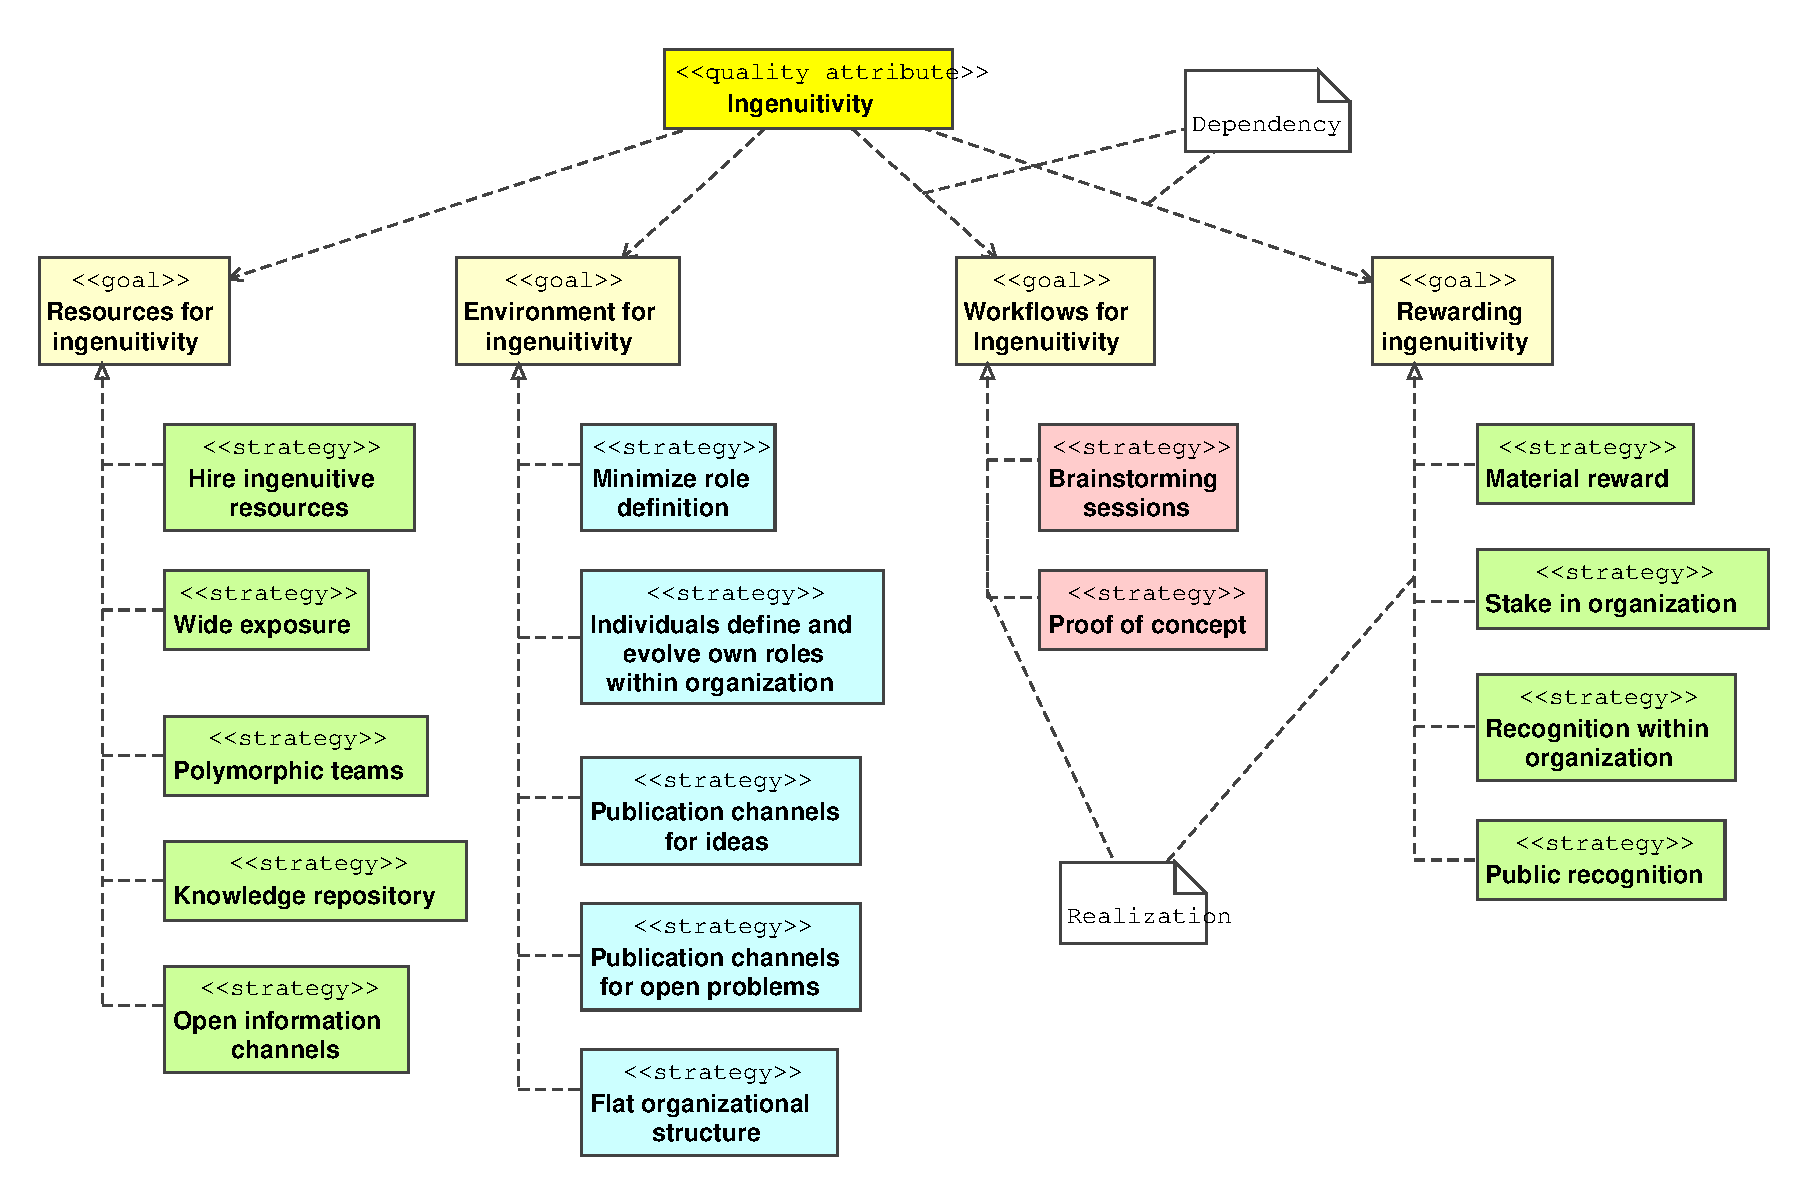
\includegraphics[scale=0.4]{ingenuitivityTactics}
    \caption{Goals and strategies for ingenuitivity}\label{ingenuitivityTactics_fig}
  \end{center}
\end{figure}


In order to achieve ingenuitivity one requires suitable resources operating in a suitable environment, workflows facilitating ingenuitivity and reward channels for ingenuitivity. Resourcing may be realized through hiring ingenuitive people, giving them wide exposure, assembling polymorphic teams, maintaining a knowledge repository and putting open information channels in place.

Strategies for providing an environment for ingenuitivity include person centric human resource management where individuals are not hired to fill specific roles, but instead define and evolve their own role within the organization, having a flat organizational structure and having information channels in place for publishing ideas and problems.

Brainstorming sessions and proof of concepts are standard and essential workflows across ingenuitive processes.

Finally one has to look at rewarding ingenuitivity. This can be done through direct financial reward, offering a stake in the company and recognizing achievements within the organization and publicly.

On the software development side, many organizations which focus on innovation use so called {\em{agile software development methodologies}}. These methodologies enforce many of the above strategies including person-centric human resourcing, polymorphic teams, open information channels, flat reporting structure, brainstorming sessions proof of concepts and minimized role definition with a tendency towards individuals defining and evolving their own roles within the organization.

\subsection{Strategies for realizing reliability}

Organizations which provide services for mission critical areas usually have reliability as one of their core quality attributes. This is a very common quality requirement in, for example, the health care and defense industries. Reliability is also used as core marketing and cost reduction strategies.

Reliability is a measure of contract compliance. If a service is not rendered according to contract then there is a failure. Failures are caused by faults in the process, but not all faults need to lead to a failure. If a fault is handled internally and the service is still rendered as per contract then we still have achieved high reliability.

Organizations which view reliability as one of their core qualities typically have to look at fault prevention, fault detection and fault recovery. Figure \ref{reliabilityTactics_fig} shows strategies commonly employed to realize these goals.

\begin{figure}[hbt]
  \begin{center}
    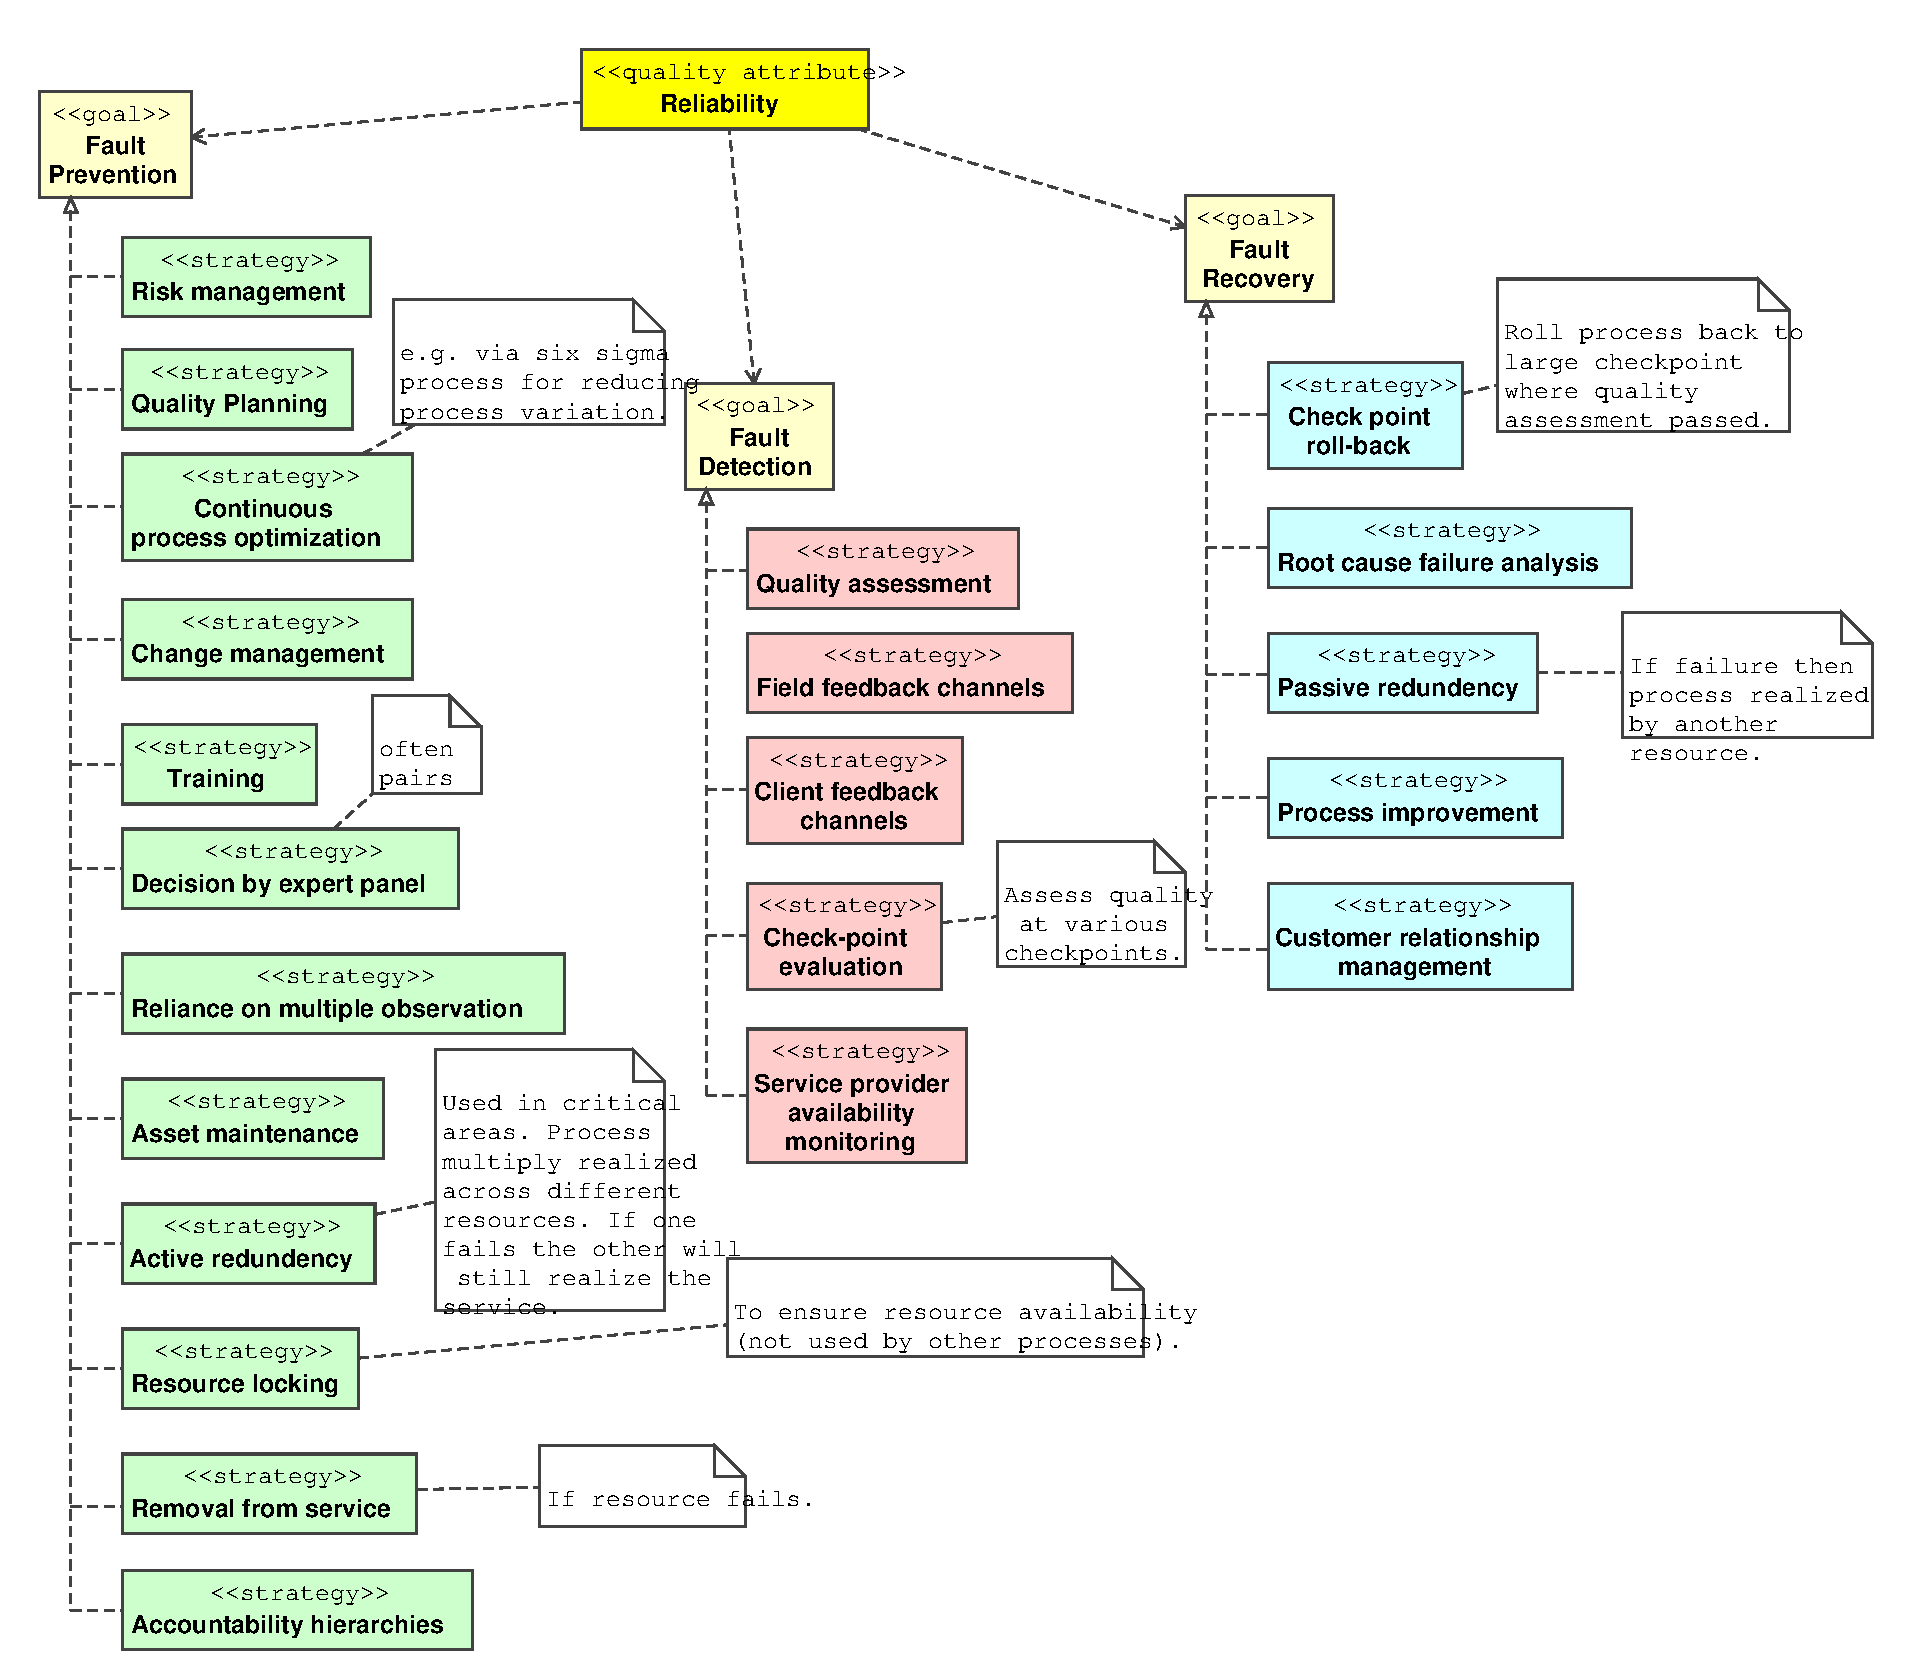
\includegraphics[scale=0.4]{reliabilityTactics}
    \caption{Goals and strategies for reliability}\label{reliabilityTactics_fig}
  \end{center}
\end{figure}


Most of the strategies are self explanatory. It may, however, be worthwhile expanding, by way of an example, on the difference between active and passive redundency. A plumbing service provider may make use of passive redundency in order to increase reliability. In that case the company may ensure that one or more plumbers remain on stand by to take over if another dispatched plumber encounters a problem (for example, if his/her vehicle breaks down). On the other hand, assume the state president has an accident. The ambulance service would most probably use active redundency, dispatching multiple vehicles concurrently. Should one vehicle encounter a problem, other vehicles are already on the way to provide the required emergency health care service. This is an example of active redundency where multiple units realize the same service concurrently and where the first or best service rendering is chosen in the end.

If reliability is your game then continuous process improvement is usually a necessity. For this organizations commonly use six sigma, a quality management approach developed by Motorola. Six sigma is meant to continuously optimize processes in order to eliminate process defects (see for example \cite{Pande-Neumann-Cavanaugh-2000}).

\subsection{Strategies for realizing flexibility}

Organization which provide customizable products and services

In \ref{flexibilityTactics_fig} we show the goals which such organizations typically set themselves in order to achieve a high level of ingenuitivity as well as some common strategies employed to realize these goals.

\begin{figure}[hbt]
  \begin{center}
    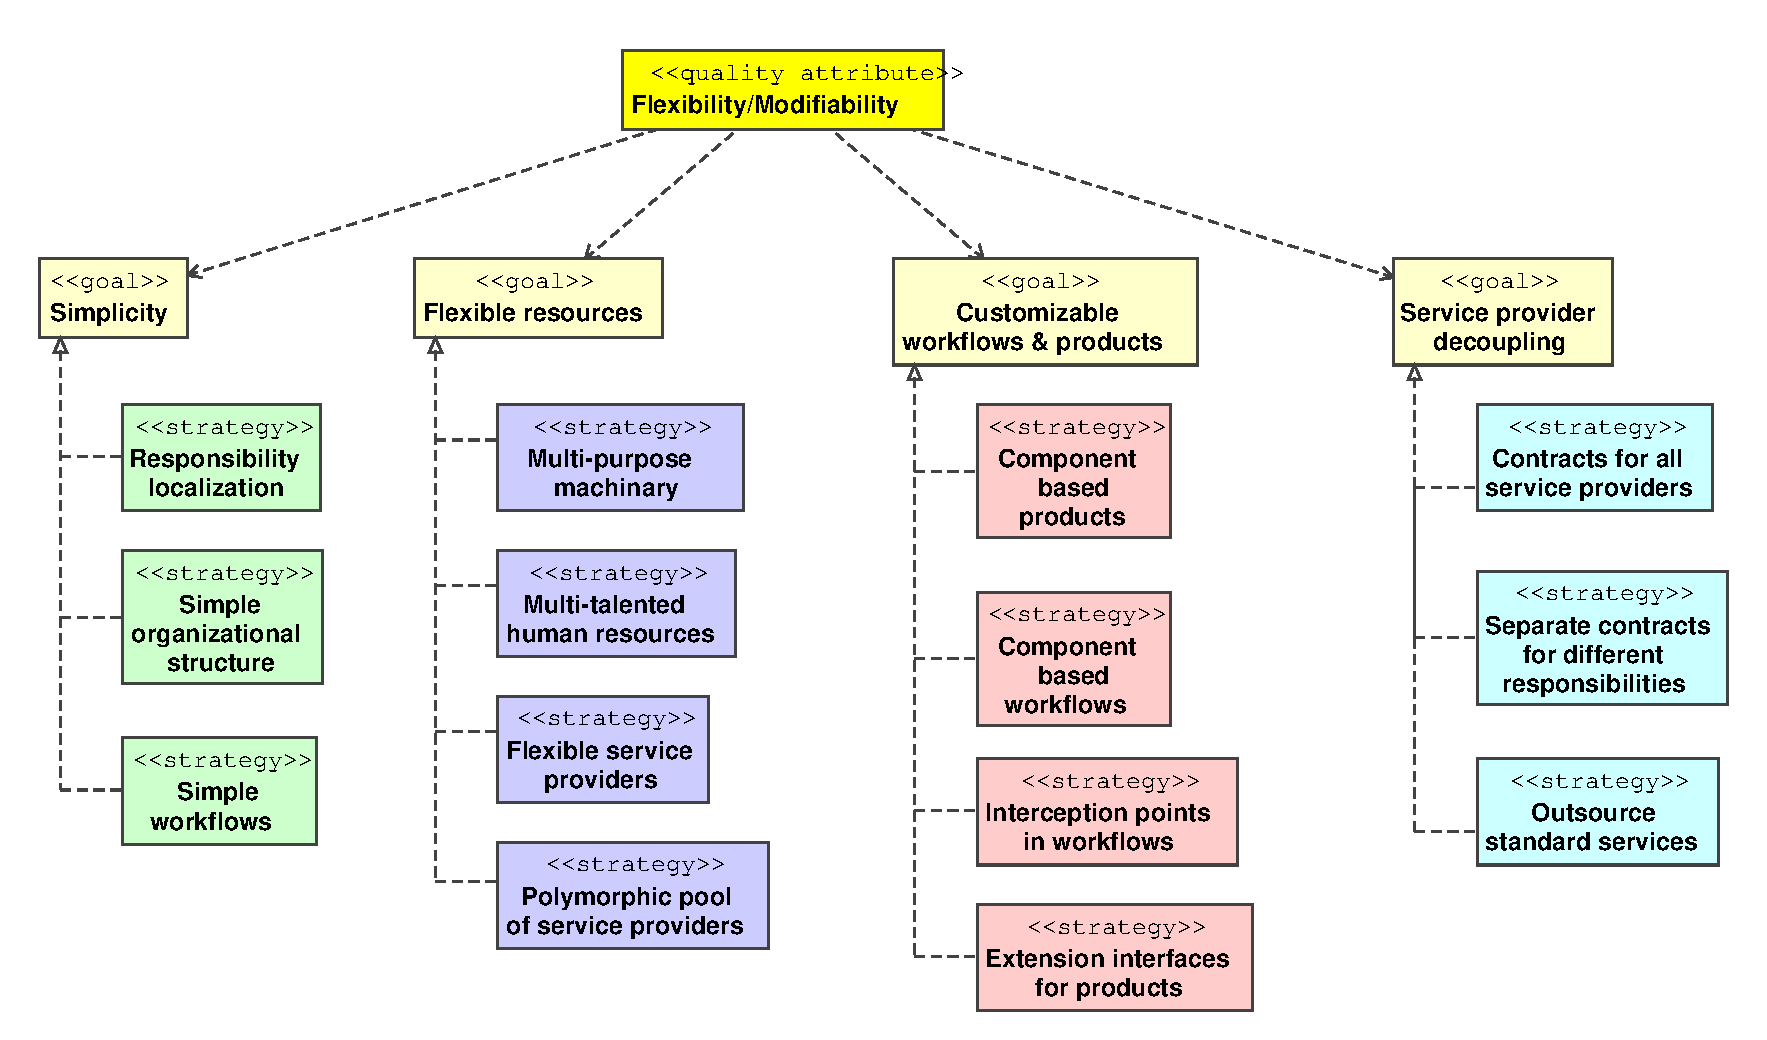
\includegraphics[scale=0.4]{flexibilityTactics}
    \caption{Goals and strategies for ingenuitivity}\label{flexibilityTactics_fig}
  \end{center}
\end{figure}

\subsection{Strategies for realizing scaleability}

Scaleability provides the ability to service/provide products to a large number of clients. This is a core quality attribute for organizations who see growth and volumes as part of their value proposition.

Organizations which want to realize an architecture supporting scaleability typically have to address the following goals: 
\begin{itemize}
  \item replicable workflows and resources (e.g.\ that they can easily set up another outlet with the same structure and workflows as other outlets),
  \item effective resource management, and
  \item infrastructure for using external resources.
\end{itemize}
\noindent  
Each of these goals can be realized through a number of strategies. Some examples are shown in figure \ref{scaleabilityTactics_fig}.

\begin{figure}[hbt]
  \begin{center}
    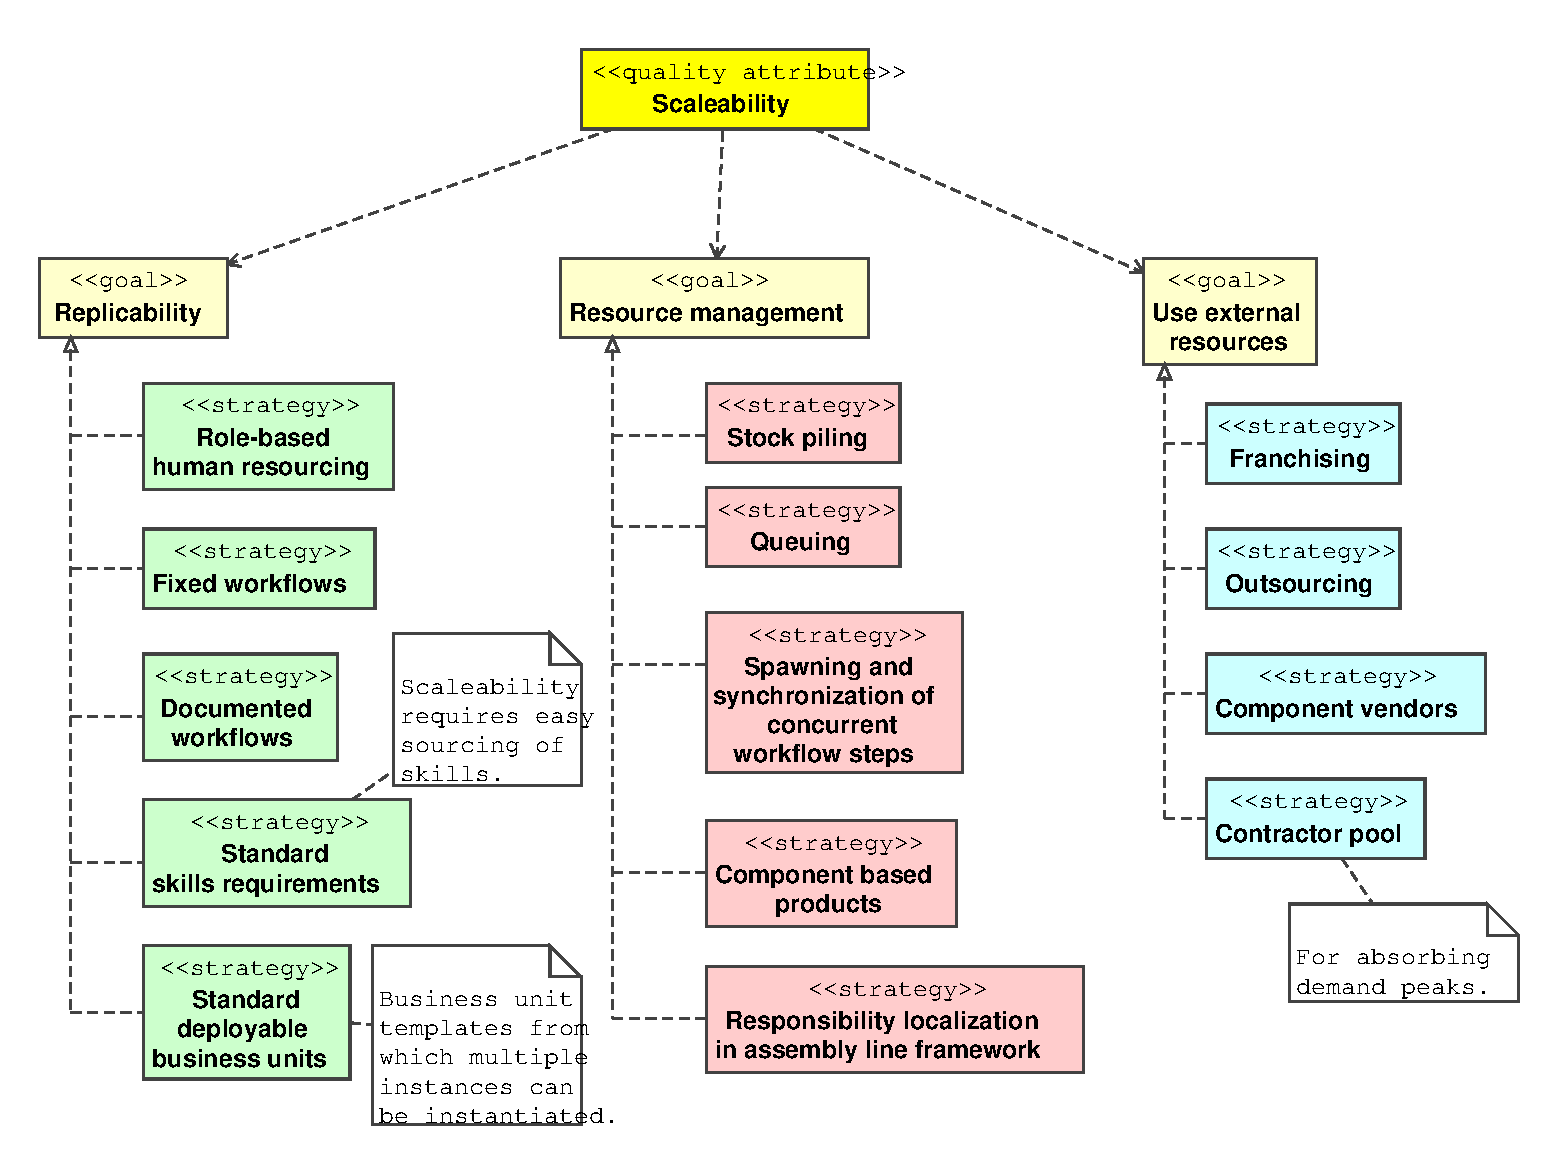
\includegraphics[scale=0.4]{scaleabilityTactics}
    \caption{Goals and strategies for scaleability}\label{scaleabilityTactics_fig}
  \end{center}
\end{figure}


\subsection{Strategies for realizing accessibility/availability}

Some organization see accessibility/availability as one of their core offerings. For example, you can purchase Coca Cola or a MacDonalds hamburger from most parts of the world. However, physical accessibility may not be required. For example, you can purchase books and music from anywhere in the world through Amazon.com. Accessibility/availability may include geographic accessibility, visibility and accessibility across time (e.g. 24x7 availability).

In \ref{accessibilityTactics_fig} we show the goals which need to be addressed for accessibility/availability and some strategies one may use in order to realize the goals.

\begin{figure}[hbt]
  \begin{center}
    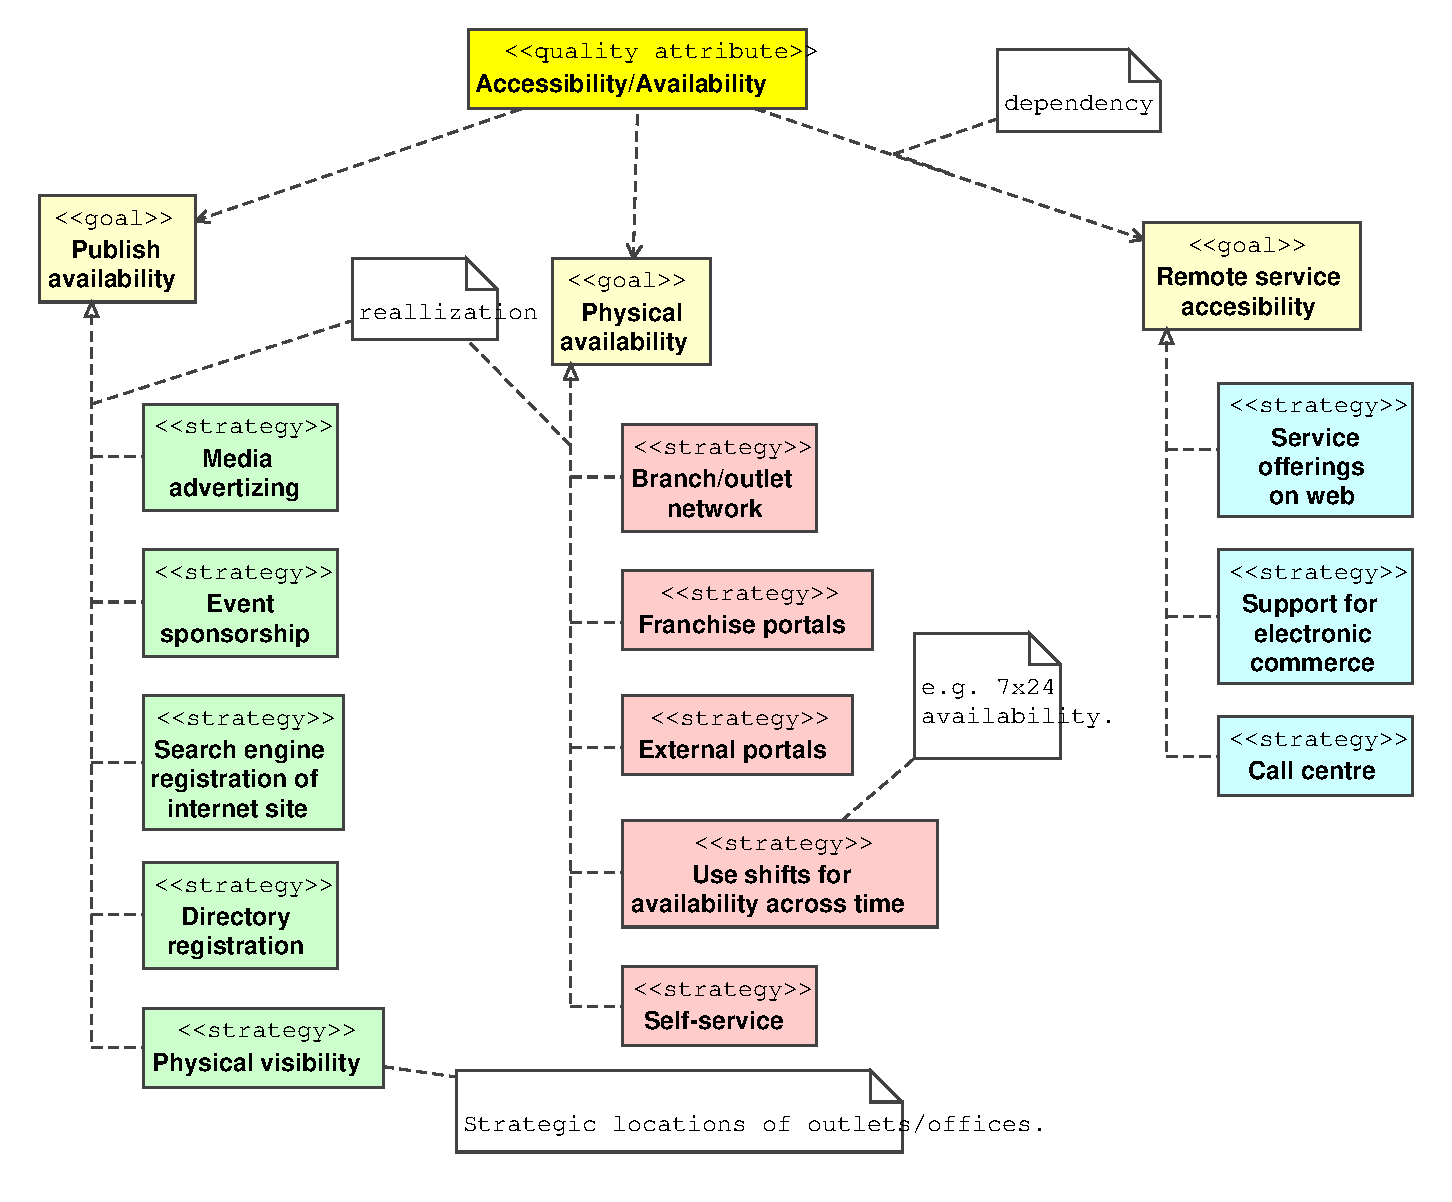
\includegraphics[scale=0.4]{accessibilityTactics}
    \caption{Goals and strategies for availability/accessibility}\label{accessibilityTactics_fig}
  \end{center}
\end{figure}

The availability of the organization's services can be published through media advertising, event sponsoring search engine and directory registration (e.g. Internet search engine, telephone book, yellow pages and other services directories as well as registration in electronic trader services like UDDI or ebXML directory services), physical visibility (choosing visible locations for outlets, branches and the head-office) and other strategies.

Some organizations aim for a high level of physical availability through extensive branch and/or outlet networks, as well as making products and/or services available through franchise and external portals. If physical availability across time is required (e.g. 24 hour availability, 7 days a week) then shift work is a standard tactic used.

\section{Example: Solms Training, Consulting \& Development}

As an example for designing an architecture around quality attributes, let us look at our own little organization, Solms Training, Consulting and Development.

\subsection{Quality drivers}

Being small we see our competitive edge mainly in the following quality attributes: 
\begin{description}
  \item[Ingenuitivity.] The ability to provide ingenuitive solutions which can assist in clients obtaining or maintaing a competitive edge.
  \item[Modifiability.] The ability to rapidly modify our service offerings to address a client's specific and changing needs.
\end{description}

\subsection{Using proven organizational patterns}

Since ingenuitivity is a central quality offering, we use the blackboard architectural pattern as the core pattern for the architecture of our little company. The ingenuitivity is thus driven by a pool of experts which solves problems collaboratively.

The blackboard-based architecture is embedded within a flat, single layer hierarchy. Auxillary supporting workflows need to be modifiable in order to effectively support the dynamic core. These are hosted within a pipes and filters based architecture managed from the flat single layer hierarchy.

\subsection{Selecting strategies for realizing our quality attributes}

Having found a suitable architectural structure, (expert pool embeded in flat hierarchy with supporting workflows provided within pipes and filters based structures), we now evaluate the strategies we can use to concretely realize our core quality attributes.

\subsubsection{Person-centric human resourcing with personal role building and evolution}

Persons are hired for their individual skills and asperations -- a person is not hired to fill a particular role within the organization. Instead experts define their own role within the organization and evolve that role over time.

\subsubsection{Wide exposure and knowledge repository}

All experts are involved in all arms of the organization, i.e. training, consulting and development. Lessons learnt in any of these are fed into the organization's knowledge repository.

The training aspect results in a structured process of deepening the organization's knowledge. The consulting adds a lateral thinking component as well as an appreciation of problems and solutions found in other organizations. The development arm provides hands-on experience and introduces a reality check for our cognitive models.

\subsubsection{Polymorphic teams}

Experts are hired to complement polymorphic teams. The combination of different formal and experience backgrounds provides fertile ground for finding novel solutions to problems.

\subsubsection{Workflow strategies for ingenuitivity}

Brainstorming sessions are central in our workflows. Ingenuitive solutions are standardly validated via proof of concepts. All acquired knowledge is fed into our knowledge repository. Course notes are assembled as compilations across available knowledge components.

\subsubsection{Rewarding ingenuitivity}

Our current reward channels for ingenuitivity include financial benefits as well as internal and public recognition. The organization is in the process of introducing ownership distribution as a further reward channel.


\section{Summary and conclusions}

The architecture is the primary vehicle through which an organization realizes its vision and core quality attributes. When designing an architecture for an organization, one can benefit from using architectural patterns which are able to effectively address certain quality attributes. The patterns are combined to provide the core infrastructure for the organization. Once this is in place, one can look at strategies which have proven that they can assist in realizing the organization's quality attributes.

The architecture provides a framework for all business processes. The business processes deployed within the architecture acquire the organizational qualities through the architecture. In this way the architecture facilitates the consistent realization of the organization's vision.

\begin{thebibliography}{99}

\bibitem[1]{Alexander-1979} {\emph{The Timeless Way of Building}}, Christopher Alexander, Oxford University Press, 1979.

\bibitem[2]{Alexander-Ishikawa-Silverstein-Jacobson-1977}
  {\emph{A Pattern Language: Towns, Buildings, Construction}}, Christopher Alexander, Sara Ishikawa, Murray Silverstein, et Max Jacobson, Oxford University Press, 1977.

\bibitem[3]{Ashmore-Henson-Chancellor-Nelson-2004}
  {\emph{Is your architecture all it can be?}}, 
Perryn Ashmore, Joel Henson, Jeff Chancellor and Mark Nelson, Business Process Trends, June 2004.

\bibitem[4]{Bass-Clements-Kazman-2003}
  {\emph{Software Architecture in Practice}}, Len Bass, Paul Clements, et Rick Kazman, Addison Wesley, 2003.

\bibitem[5]{Brickley-Smith-Zimmermann-2001}
  {\emph{Managerial Economics and Organizational Architecture}}, 
	James Brickley, Clifford W. Smith, et Jerold Zimmermann, McGraw-Hill, 2001.

\bibitem[6]{Ethiraj-Levinthal-2004}
  {\emph{Modularity and innovation in complex systems}}, Sendil K. Ethiraj and
Daniel Levinthal, Management Science, vol. 50, 159-173, 2004.

\bibitem[7]{Frankel-2003}{\emph{Model Driven Architecture: Applying MDA to enterprise computing}}, David S. Frankel, John Wiley \& Sons, 2003.

\bibitem[8]{Galbraith-Downy-Kates-2001}
  {\emph{Designing Dynamic Organizations: A Hands-On Guide for Leaders at All Levels}}, 
	Jay Galbraith, Diane Downy, et Amy Kates, American Management Association, November 2001.

\bibitem[9]{Gamma-Helm-Johnson-Vlissides-1995}
  {\emph{Design Patterns}}, 
  Erich Gamma, Richard Helm, Ralph Johnson, et John Vlissides, Addison-Wesley, 1995.

\bibitem[10]{Harris-Raviv-2002}
  {\emph{Organization Design}}, Milton Harris and Artur Raviv, Management Science,
  vol 48 no 7, 852-865, 2002.

\bibitem[11]{Kazman-1994}
  {\emph{Toward Deriving Software Architectures from Attributes}}, Rick Katzman, 1994.

\bibitem[12]{King-1995}
  {\emph{Creating a strategic capabilities architectures}}, W. R. King,
  Information System Management, vol 12 no 1, 67-69, 1995.

\bibitem[13]{Leavitt-2004}
  {\emph{Why Hierarchies Are Here to Stay and How to Manage Them More Effectively}}, 
  Harold J. Leavitt, Harvard Business School Press, November 2004.

\bibitem[14]{Morabito-Sack-Bhate-1999}
  {\emph{Organization Modeling}}, 
  Joseph Morabito, Ira Sack, et Anilkumar Bhate, Prentice Hall, 1999.

\bibitem[15]{Nadler-Gerstein-Shaw-1992}
  {\emph{Organizational Architecture}}, 
  David A. Nadler, Marc C. Gerstein, et Robert B. Shaw, Jossey-Bass, May 1992.

\bibitem[16]{Pande-Neumann-Cavanaugh-2000}
  {\emph{The Six Sigma Way}}, 
  P.S. Pande, R.P. Neumann, \& R.R. Cavanaugh, McGraw-Hill, 2000.

\bibitem[17]{Schonberger-1982}
  {\emph{Japanese Manufacturing Techniques}}, 
  Richard J. Schonberger, Free Press, 1982.


\end{thebibliography}

\end{document}
